\batchmode
\documentclass[twoside]{article}

% Packages required by doxygen
\usepackage{fixltx2e}
\usepackage{calc}
\usepackage{doxygen}
\usepackage[export]{adjustbox} % also loads graphicx
\usepackage{graphicx}
\usepackage[utf8]{inputenc}
\usepackage{makeidx}
\usepackage{multicol}
\usepackage{multirow}
\PassOptionsToPackage{warn}{textcomp}
\usepackage{textcomp}
\usepackage[nointegrals]{wasysym}
\usepackage[table]{xcolor}

% Font selection
\usepackage[T1]{fontenc}
\usepackage[scaled=.90]{helvet}
\usepackage{courier}
\usepackage{amssymb}
\usepackage{sectsty}
\renewcommand{\familydefault}{\sfdefault}
\allsectionsfont{%
  \fontseries{bc}\selectfont%
  \color{darkgray}%
}
\renewcommand{\DoxyLabelFont}{%
  \fontseries{bc}\selectfont%
  \color{darkgray}%
}
\newcommand{\+}{\discretionary{\mbox{\scriptsize$\hookleftarrow$}}{}{}}

% Page & text layout
\usepackage{geometry}
\geometry{%
  letterpaper,%
  top=2.5cm,%
  bottom=2.5cm,%
  left=2.5cm,%
  right=2.5cm%
}
\tolerance=750
\hfuzz=15pt
\hbadness=750
\setlength{\emergencystretch}{15pt}
\setlength{\parindent}{0cm}
\setlength{\parskip}{3ex plus 2ex minus 2ex}
\makeatletter
\renewcommand{\paragraph}{%
  \@startsection{paragraph}{4}{0ex}{-1.0ex}{1.0ex}{%
    \normalfont\normalsize\bfseries\SS@parafont%
  }%
}
\renewcommand{\subparagraph}{%
  \@startsection{subparagraph}{5}{0ex}{-1.0ex}{1.0ex}{%
    \normalfont\normalsize\bfseries\SS@subparafont%
  }%
}
\makeatother

% Headers & footers
\usepackage{fancyhdr}
\pagestyle{fancyplain}
\fancyhead[LE]{\fancyplain{}{\bfseries\thepage}}
\fancyhead[CE]{\fancyplain{}{}}
\fancyhead[RE]{\fancyplain{}{\bfseries\leftmark}}
\fancyhead[LO]{\fancyplain{}{\bfseries\rightmark}}
\fancyhead[CO]{\fancyplain{}{}}
\fancyhead[RO]{\fancyplain{}{\bfseries\thepage}}
\fancyfoot[LE]{\fancyplain{}{}}
\fancyfoot[CE]{\fancyplain{}{}}
\fancyfoot[RE]{\fancyplain{}{\bfseries\scriptsize Generated by Doxygen }}
\fancyfoot[LO]{\fancyplain{}{\bfseries\scriptsize Generated by Doxygen }}
\fancyfoot[CO]{\fancyplain{}{}}
\fancyfoot[RO]{\fancyplain{}{}}
\renewcommand{\footrulewidth}{0.4pt}
\renewcommand{\sectionmark}[1]{%
  \markright{\thesection\ #1}%
}

% Indices & bibliography
\usepackage{natbib}
\usepackage[titles]{tocloft}
\setcounter{tocdepth}{3}
\setcounter{secnumdepth}{5}
\makeindex

% Hyperlinks (required, but should be loaded last)
\usepackage{ifpdf}
\ifpdf
  \usepackage[pdftex,pagebackref=true]{hyperref}
\else
  \usepackage[ps2pdf,pagebackref=true]{hyperref}
\fi
\hypersetup{%
  colorlinks=true,%
  linkcolor=blue,%
  citecolor=blue,%
  unicode%
}

% Custom commands
\newcommand{\clearemptydoublepage}{%
  \newpage{\pagestyle{empty}\cleardoublepage}%
}

\usepackage{caption}
\captionsetup{labelsep=space,justification=centering,font={bf},singlelinecheck=off,skip=4pt,position=top}

%===== C O N T E N T S =====

\begin{document}

% Titlepage & ToC
\hypersetup{pageanchor=false,
             bookmarksnumbered=true,
             pdfencoding=unicode
            }
\pagenumbering{roman}
\begin{titlepage}
\vspace*{7cm}
\begin{center}%
{\Large S\+R\+Render }\\
\vspace*{1cm}
{\large Generated by Doxygen 1.8.11}\\
\end{center}
\end{titlepage}
\tableofcontents
\pagenumbering{arabic}
\hypersetup{pageanchor=true}

%--- Begin generated contents ---
\section{S\+R\+Render}
\label{index}\hypertarget{index}{}Super-\/resolution microscopy parallel rendering tool for Matlab and C++.

\subsubsection*{L\+I\+C\+E\+N\+SE}


\begin{DoxyItemize}
\item Copyright\+: 2014-\/2019
\item Author\+: Mark J. Olah
\item Email\+: (\href{mailto:mjo@cs.unm}{\tt mjo@cs.\+unm} D\+OT edu)
\item L\+I\+C\+E\+N\+SE\+: Apache 2.\+0. See \href{https://github.com/markjolah/Tracker/blob/master/LICENSE}{\tt L\+I\+C\+E\+N\+SE} file. 
\end{DoxyItemize}
\section{Namespace Index}
\subsection{Namespace List}
Here is a list of all namespaces with brief descriptions\+:\begin{DoxyCompactList}
\item\contentsline{section}{\hyperlink{namespacesrrender}{srrender} }{\pageref{namespacesrrender}}{}
\end{DoxyCompactList}

\section{Class Index}
\subsection{Class List}
Here are the classes, structs, unions and interfaces with brief descriptions\+:\begin{DoxyCompactList}
\item\contentsline{section}{\hyperlink{classsrrender_1_1SRRender2D}{srrender\+::\+S\+R\+Render2\+D$<$ Float\+T, Idx\+T $>$} }{\pageref{classsrrender_1_1SRRender2D}}{}
\end{DoxyCompactList}

\section{File Index}
\subsection{File List}
Here is a list of all files with brief descriptions\+:\begin{DoxyCompactList}
\item\contentsline{section}{\hyperlink{SRRender_8h}{S\+R\+Render.\+h} \\*The class declaration and inline and templated functions for S\+R\+Render }{\pageref{SRRender_8h}}{}
\end{DoxyCompactList}

\section{Namespace Documentation}
\hypertarget{namespacesrrender}{}\subsection{srrender Namespace Reference}
\label{namespacesrrender}\index{srrender@{srrender}}
\subsubsection*{Classes}
\begin{DoxyCompactItemize}
\item 
class \hyperlink{classsrrender_1_1SRRender2D}{S\+R\+Render2D}
\end{DoxyCompactItemize}
\subsubsection*{Typedefs}
\begin{DoxyCompactItemize}
\item 
using \hyperlink{namespacesrrender_a9a142db9660e71c105d0ea15f96ff6b2}{S\+R\+Render\+Error} = backtrace\+\_\+exception\+::\+Backtrace\+Exception
\end{DoxyCompactItemize}


\subsubsection{Typedef Documentation}
\index{srrender@{srrender}!S\+R\+Render\+Error@{S\+R\+Render\+Error}}
\index{S\+R\+Render\+Error@{S\+R\+Render\+Error}!srrender@{srrender}}
\paragraph[{\texorpdfstring{S\+R\+Render\+Error}{SRRenderError}}]{\setlength{\rightskip}{0pt plus 5cm}using {\bf srrender\+::\+S\+R\+Render\+Error} = typedef backtrace\+\_\+exception\+::\+Backtrace\+Exception}\hypertarget{namespacesrrender_a9a142db9660e71c105d0ea15f96ff6b2}{}\label{namespacesrrender_a9a142db9660e71c105d0ea15f96ff6b2}


Definition at line 17 of file S\+R\+Render.\+h.


\section{Class Documentation}
\hypertarget{classsrrender_1_1SRRender2D}{}\subsection{srrender\+:\+:S\+R\+Render2D$<$ FloatT, IdxT $>$ Class Template Reference}
\label{classsrrender_1_1SRRender2D}\index{srrender\+::\+S\+R\+Render2\+D$<$ Float\+T, Idx\+T $>$@{srrender\+::\+S\+R\+Render2\+D$<$ Float\+T, Idx\+T $>$}}


{\ttfamily \#include $<$/home/travis/build/markjolah/\+S\+R\+Render/include/\+S\+R\+Render/\+S\+R\+Render.\+h$>$}

\subsubsection*{Public Types}
\begin{DoxyCompactItemize}
\item 
using \hyperlink{classsrrender_1_1SRRender2D_abf2e65ab6bcf77af73d3988cc3d457b9}{I\+VecT} = arma\+::\+Col$<$ IdxT $>$
\item 
using \hyperlink{classsrrender_1_1SRRender2D_ab2b17bb30a0f86d610ef90e2e8e97e25}{VecT} = arma\+::\+Col$<$ FloatT $>$
\item 
using \hyperlink{classsrrender_1_1SRRender2D_a84ba69a439ee39a97bb8fed4eebac011}{ImageT} = arma\+::\+Mat$<$ FloatT $>$
\item 
using \hyperlink{classsrrender_1_1SRRender2D_a884febde0e56f7e07fd470f2498eadbd}{MovieT} = arma\+::\+Cube$<$ FloatT $>$
\item 
using \hyperlink{classsrrender_1_1SRRender2D_ac2433ed86b4b21ff082ba8c2a080e26a}{Emitter\+VecT} = arma\+::\+Mat$<$ FloatT $>$
\end{DoxyCompactItemize}
\subsubsection*{Static Public Member Functions}
\begin{DoxyCompactItemize}
\item 
static void \hyperlink{classsrrender_1_1SRRender2D_a2e1dcc7e39a16514a4b3f1226c0610f5}{render\+Hist} (const \hyperlink{classsrrender_1_1SRRender2D_ac2433ed86b4b21ff082ba8c2a080e26a}{Emitter\+VecT} \&points, const \hyperlink{classsrrender_1_1SRRender2D_ab2b17bb30a0f86d610ef90e2e8e97e25}{VecT} \&roi, \hyperlink{classsrrender_1_1SRRender2D_a84ba69a439ee39a97bb8fed4eebac011}{ImageT} \&im)
\item 
static void \hyperlink{classsrrender_1_1SRRender2D_ac3b2d60e4a9d86950938db63a57b5639}{render\+Gauss} (const \hyperlink{classsrrender_1_1SRRender2D_ac2433ed86b4b21ff082ba8c2a080e26a}{Emitter\+VecT} \&points, const \hyperlink{classsrrender_1_1SRRender2D_ab2b17bb30a0f86d610ef90e2e8e97e25}{VecT} \&roi, \hyperlink{classsrrender_1_1SRRender2D_a84ba69a439ee39a97bb8fed4eebac011}{ImageT} \&im, FloatT sigma\+Accuracy=\hyperlink{classsrrender_1_1SRRender2D_ac1a7fcf709ff55bf7b70e91fff12cce8}{Default\+Sigma\+Accuracy})
\item 
static void \hyperlink{classsrrender_1_1SRRender2D_a8d72c884651325fdf6afa19ad025a877}{render\+Hist\+Movie} (const \hyperlink{classsrrender_1_1SRRender2D_ac2433ed86b4b21ff082ba8c2a080e26a}{Emitter\+VecT} \&points, const \hyperlink{classsrrender_1_1SRRender2D_ab2b17bb30a0f86d610ef90e2e8e97e25}{VecT} \&roi, \hyperlink{classsrrender_1_1SRRender2D_a884febde0e56f7e07fd470f2498eadbd}{MovieT} \&im)
\item 
static void \hyperlink{classsrrender_1_1SRRender2D_ae392b80afdf6dee6d85dd84343dfa7e6}{render\+Gauss\+Movie} (const \hyperlink{classsrrender_1_1SRRender2D_ac2433ed86b4b21ff082ba8c2a080e26a}{Emitter\+VecT} \&points, const \hyperlink{classsrrender_1_1SRRender2D_ab2b17bb30a0f86d610ef90e2e8e97e25}{VecT} \&roi, \hyperlink{classsrrender_1_1SRRender2D_a884febde0e56f7e07fd470f2498eadbd}{MovieT} \&im, FloatT sigma\+Accuracy=\hyperlink{classsrrender_1_1SRRender2D_ac1a7fcf709ff55bf7b70e91fff12cce8}{Default\+Sigma\+Accuracy})
\end{DoxyCompactItemize}
\subsubsection*{Static Public Attributes}
\begin{DoxyCompactItemize}
\item 
static const FloatT \hyperlink{classsrrender_1_1SRRender2D_ac1a7fcf709ff55bf7b70e91fff12cce8}{Default\+Sigma\+Accuracy}
\end{DoxyCompactItemize}


\subsubsection{Detailed Description}
\subsubsection*{template$<$class FloatT = float, class IdxT = uint32\+\_\+t$>$\\*
class srrender\+::\+S\+R\+Render2\+D$<$ Float\+T, Idx\+T $>$}

Points format. Row-\/oriented each row is a point, each column is a property 2D render\+Hist Columns\+: \mbox{[}I X Y\mbox{]} 2D render\+Gauss Columns\+:\mbox{[}I X Y sigmaX sigmaY\mbox{]} 2D render\+Hist\+Movie Columns\+: \mbox{[}I X Y Frame\mbox{]} -\/ Frame is 0-\/indexed 2D render\+Gauss\+Movie Columns\+:\mbox{[}I X Y sigmaX sigmaY Frame\mbox{]} -\/ Frame is 0-\/indexed

The \textquotesingle{}size\textquotesingle{} parameter gives the size of the entire field of view to be rendered in units corresponding to the points format vectors. 

Definition at line 32 of file S\+R\+Render.\+h.



\subsubsection{Member Typedef Documentation}
\index{srrender\+::\+S\+R\+Render2D@{srrender\+::\+S\+R\+Render2D}!Emitter\+VecT@{Emitter\+VecT}}
\index{Emitter\+VecT@{Emitter\+VecT}!srrender\+::\+S\+R\+Render2D@{srrender\+::\+S\+R\+Render2D}}
\paragraph[{\texorpdfstring{Emitter\+VecT}{EmitterVecT}}]{\setlength{\rightskip}{0pt plus 5cm}template$<$class FloatT  = float, class IdxT  = uint32\+\_\+t$>$ using {\bf srrender\+::\+S\+R\+Render2D}$<$ FloatT, IdxT $>$\+::{\bf Emitter\+VecT} =  arma\+::\+Mat$<$FloatT$>$}\hypertarget{classsrrender_1_1SRRender2D_ac2433ed86b4b21ff082ba8c2a080e26a}{}\label{classsrrender_1_1SRRender2D_ac2433ed86b4b21ff082ba8c2a080e26a}


Definition at line 38 of file S\+R\+Render.\+h.

\index{srrender\+::\+S\+R\+Render2D@{srrender\+::\+S\+R\+Render2D}!ImageT@{ImageT}}
\index{ImageT@{ImageT}!srrender\+::\+S\+R\+Render2D@{srrender\+::\+S\+R\+Render2D}}
\paragraph[{\texorpdfstring{ImageT}{ImageT}}]{\setlength{\rightskip}{0pt plus 5cm}template$<$class FloatT  = float, class IdxT  = uint32\+\_\+t$>$ using {\bf srrender\+::\+S\+R\+Render2D}$<$ FloatT, IdxT $>$\+::{\bf ImageT} =  arma\+::\+Mat$<$FloatT$>$}\hypertarget{classsrrender_1_1SRRender2D_a84ba69a439ee39a97bb8fed4eebac011}{}\label{classsrrender_1_1SRRender2D_a84ba69a439ee39a97bb8fed4eebac011}


Definition at line 36 of file S\+R\+Render.\+h.

\index{srrender\+::\+S\+R\+Render2D@{srrender\+::\+S\+R\+Render2D}!I\+VecT@{I\+VecT}}
\index{I\+VecT@{I\+VecT}!srrender\+::\+S\+R\+Render2D@{srrender\+::\+S\+R\+Render2D}}
\paragraph[{\texorpdfstring{I\+VecT}{IVecT}}]{\setlength{\rightskip}{0pt plus 5cm}template$<$class FloatT  = float, class IdxT  = uint32\+\_\+t$>$ using {\bf srrender\+::\+S\+R\+Render2D}$<$ FloatT, IdxT $>$\+::{\bf I\+VecT} =  arma\+::\+Col$<$IdxT$>$}\hypertarget{classsrrender_1_1SRRender2D_abf2e65ab6bcf77af73d3988cc3d457b9}{}\label{classsrrender_1_1SRRender2D_abf2e65ab6bcf77af73d3988cc3d457b9}


Definition at line 34 of file S\+R\+Render.\+h.

\index{srrender\+::\+S\+R\+Render2D@{srrender\+::\+S\+R\+Render2D}!MovieT@{MovieT}}
\index{MovieT@{MovieT}!srrender\+::\+S\+R\+Render2D@{srrender\+::\+S\+R\+Render2D}}
\paragraph[{\texorpdfstring{MovieT}{MovieT}}]{\setlength{\rightskip}{0pt plus 5cm}template$<$class FloatT  = float, class IdxT  = uint32\+\_\+t$>$ using {\bf srrender\+::\+S\+R\+Render2D}$<$ FloatT, IdxT $>$\+::{\bf MovieT} =  arma\+::\+Cube$<$FloatT$>$}\hypertarget{classsrrender_1_1SRRender2D_a884febde0e56f7e07fd470f2498eadbd}{}\label{classsrrender_1_1SRRender2D_a884febde0e56f7e07fd470f2498eadbd}


Definition at line 37 of file S\+R\+Render.\+h.

\index{srrender\+::\+S\+R\+Render2D@{srrender\+::\+S\+R\+Render2D}!VecT@{VecT}}
\index{VecT@{VecT}!srrender\+::\+S\+R\+Render2D@{srrender\+::\+S\+R\+Render2D}}
\paragraph[{\texorpdfstring{VecT}{VecT}}]{\setlength{\rightskip}{0pt plus 5cm}template$<$class FloatT  = float, class IdxT  = uint32\+\_\+t$>$ using {\bf srrender\+::\+S\+R\+Render2D}$<$ FloatT, IdxT $>$\+::{\bf VecT} =  arma\+::\+Col$<$FloatT$>$}\hypertarget{classsrrender_1_1SRRender2D_ab2b17bb30a0f86d610ef90e2e8e97e25}{}\label{classsrrender_1_1SRRender2D_ab2b17bb30a0f86d610ef90e2e8e97e25}


Definition at line 35 of file S\+R\+Render.\+h.



\subsubsection{Member Function Documentation}
\index{srrender\+::\+S\+R\+Render2D@{srrender\+::\+S\+R\+Render2D}!render\+Gauss@{render\+Gauss}}
\index{render\+Gauss@{render\+Gauss}!srrender\+::\+S\+R\+Render2D@{srrender\+::\+S\+R\+Render2D}}
\paragraph[{\texorpdfstring{render\+Gauss(const Emitter\+Vec\+T \&points, const Vec\+T \&roi, Image\+T \&im, Float\+T sigma\+Accuracy=\+Default\+Sigma\+Accuracy)}{renderGauss(const EmitterVecT &points, const VecT &roi, ImageT &im, FloatT sigmaAccuracy=DefaultSigmaAccuracy)}}]{\setlength{\rightskip}{0pt plus 5cm}template$<$class FloatT  = float, class IdxT  = uint32\+\_\+t$>$ static void {\bf srrender\+::\+S\+R\+Render2D}$<$ FloatT, IdxT $>$\+::render\+Gauss (
\begin{DoxyParamCaption}
\item[{const {\bf Emitter\+VecT} \&}]{points, }
\item[{const {\bf VecT} \&}]{roi, }
\item[{{\bf ImageT} \&}]{im, }
\item[{FloatT}]{sigma\+Accuracy = {\ttfamily {\bf Default\+Sigma\+Accuracy}}}
\end{DoxyParamCaption}
)\hspace{0.3cm}{\ttfamily [static]}}\hypertarget{classsrrender_1_1SRRender2D_ac3b2d60e4a9d86950938db63a57b5639}{}\label{classsrrender_1_1SRRender2D_ac3b2d60e4a9d86950938db63a57b5639}
\index{srrender\+::\+S\+R\+Render2D@{srrender\+::\+S\+R\+Render2D}!render\+Gauss\+Movie@{render\+Gauss\+Movie}}
\index{render\+Gauss\+Movie@{render\+Gauss\+Movie}!srrender\+::\+S\+R\+Render2D@{srrender\+::\+S\+R\+Render2D}}
\paragraph[{\texorpdfstring{render\+Gauss\+Movie(const Emitter\+Vec\+T \&points, const Vec\+T \&roi, Movie\+T \&im, Float\+T sigma\+Accuracy=\+Default\+Sigma\+Accuracy)}{renderGaussMovie(const EmitterVecT &points, const VecT &roi, MovieT &im, FloatT sigmaAccuracy=DefaultSigmaAccuracy)}}]{\setlength{\rightskip}{0pt plus 5cm}template$<$class FloatT  = float, class IdxT  = uint32\+\_\+t$>$ static void {\bf srrender\+::\+S\+R\+Render2D}$<$ FloatT, IdxT $>$\+::render\+Gauss\+Movie (
\begin{DoxyParamCaption}
\item[{const {\bf Emitter\+VecT} \&}]{points, }
\item[{const {\bf VecT} \&}]{roi, }
\item[{{\bf MovieT} \&}]{im, }
\item[{FloatT}]{sigma\+Accuracy = {\ttfamily {\bf Default\+Sigma\+Accuracy}}}
\end{DoxyParamCaption}
)\hspace{0.3cm}{\ttfamily [static]}}\hypertarget{classsrrender_1_1SRRender2D_ae392b80afdf6dee6d85dd84343dfa7e6}{}\label{classsrrender_1_1SRRender2D_ae392b80afdf6dee6d85dd84343dfa7e6}
\index{srrender\+::\+S\+R\+Render2D@{srrender\+::\+S\+R\+Render2D}!render\+Hist@{render\+Hist}}
\index{render\+Hist@{render\+Hist}!srrender\+::\+S\+R\+Render2D@{srrender\+::\+S\+R\+Render2D}}
\paragraph[{\texorpdfstring{render\+Hist(const Emitter\+Vec\+T \&points, const Vec\+T \&roi, Image\+T \&im)}{renderHist(const EmitterVecT &points, const VecT &roi, ImageT &im)}}]{\setlength{\rightskip}{0pt plus 5cm}template$<$class FloatT  = float, class IdxT  = uint32\+\_\+t$>$ static void {\bf srrender\+::\+S\+R\+Render2D}$<$ FloatT, IdxT $>$\+::render\+Hist (
\begin{DoxyParamCaption}
\item[{const {\bf Emitter\+VecT} \&}]{points, }
\item[{const {\bf VecT} \&}]{roi, }
\item[{{\bf ImageT} \&}]{im}
\end{DoxyParamCaption}
)\hspace{0.3cm}{\ttfamily [static]}}\hypertarget{classsrrender_1_1SRRender2D_a2e1dcc7e39a16514a4b3f1226c0610f5}{}\label{classsrrender_1_1SRRender2D_a2e1dcc7e39a16514a4b3f1226c0610f5}
\index{srrender\+::\+S\+R\+Render2D@{srrender\+::\+S\+R\+Render2D}!render\+Hist\+Movie@{render\+Hist\+Movie}}
\index{render\+Hist\+Movie@{render\+Hist\+Movie}!srrender\+::\+S\+R\+Render2D@{srrender\+::\+S\+R\+Render2D}}
\paragraph[{\texorpdfstring{render\+Hist\+Movie(const Emitter\+Vec\+T \&points, const Vec\+T \&roi, Movie\+T \&im)}{renderHistMovie(const EmitterVecT &points, const VecT &roi, MovieT &im)}}]{\setlength{\rightskip}{0pt plus 5cm}template$<$class FloatT  = float, class IdxT  = uint32\+\_\+t$>$ static void {\bf srrender\+::\+S\+R\+Render2D}$<$ FloatT, IdxT $>$\+::render\+Hist\+Movie (
\begin{DoxyParamCaption}
\item[{const {\bf Emitter\+VecT} \&}]{points, }
\item[{const {\bf VecT} \&}]{roi, }
\item[{{\bf MovieT} \&}]{im}
\end{DoxyParamCaption}
)\hspace{0.3cm}{\ttfamily [static]}}\hypertarget{classsrrender_1_1SRRender2D_a8d72c884651325fdf6afa19ad025a877}{}\label{classsrrender_1_1SRRender2D_a8d72c884651325fdf6afa19ad025a877}


\subsubsection{Member Data Documentation}
\index{srrender\+::\+S\+R\+Render2D@{srrender\+::\+S\+R\+Render2D}!Default\+Sigma\+Accuracy@{Default\+Sigma\+Accuracy}}
\index{Default\+Sigma\+Accuracy@{Default\+Sigma\+Accuracy}!srrender\+::\+S\+R\+Render2D@{srrender\+::\+S\+R\+Render2D}}
\paragraph[{\texorpdfstring{Default\+Sigma\+Accuracy}{DefaultSigmaAccuracy}}]{\setlength{\rightskip}{0pt plus 5cm}template$<$class FloatT  = float, class IdxT  = uint32\+\_\+t$>$ const FloatT {\bf srrender\+::\+S\+R\+Render2D}$<$ FloatT, IdxT $>$\+::Default\+Sigma\+Accuracy\hspace{0.3cm}{\ttfamily [static]}}\hypertarget{classsrrender_1_1SRRender2D_ac1a7fcf709ff55bf7b70e91fff12cce8}{}\label{classsrrender_1_1SRRender2D_ac1a7fcf709ff55bf7b70e91fff12cce8}


Definition at line 39 of file S\+R\+Render.\+h.



The documentation for this class was generated from the following file\+:\begin{DoxyCompactItemize}
\item 
\hyperlink{SRRender_8h}{S\+R\+Render.\+h}\end{DoxyCompactItemize}

\section{File Documentation}
\hypertarget{README_8md}{}\subsection{R\+E\+A\+D\+M\+E.\+md File Reference}
\label{README_8md}\index{R\+E\+A\+D\+M\+E.\+md@{R\+E\+A\+D\+M\+E.\+md}}

\hypertarget{SRRender_8h}{}\subsection{S\+R\+Render.\+h File Reference}
\label{SRRender_8h}\index{S\+R\+Render.\+h@{S\+R\+Render.\+h}}


The class declaration and inline and templated functions for S\+R\+Render.  


{\ttfamily \#include $<$Backtrace\+Exception/\+Backtrace\+Exception.\+h$>$}\\*
{\ttfamily \#include $<$armadillo$>$}\\*
Include dependency graph for S\+R\+Render.\+h\+:\nopagebreak
\begin{figure}[H]
\begin{center}
\leavevmode
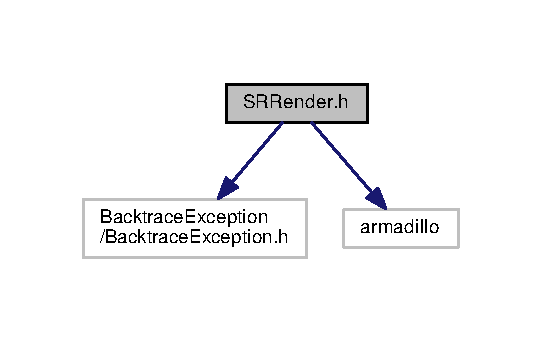
\includegraphics[width=260pt]{SRRender_8h__incl}
\end{center}
\end{figure}
\subsubsection*{Classes}
\begin{DoxyCompactItemize}
\item 
class \hyperlink{classsrrender_1_1SRRender2D}{srrender\+::\+S\+R\+Render2\+D$<$ Float\+T, Idx\+T $>$}
\end{DoxyCompactItemize}
\subsubsection*{Namespaces}
\begin{DoxyCompactItemize}
\item 
 \hyperlink{namespacesrrender}{srrender}
\end{DoxyCompactItemize}
\subsubsection*{Typedefs}
\begin{DoxyCompactItemize}
\item 
using \hyperlink{namespacesrrender_a9a142db9660e71c105d0ea15f96ff6b2}{srrender\+::\+S\+R\+Render\+Error} = backtrace\+\_\+exception\+::\+Backtrace\+Exception
\end{DoxyCompactItemize}


\subsubsection{Detailed Description}
The class declaration and inline and templated functions for S\+R\+Render. 

\begin{DoxyAuthor}{Author}
Mark J. Olah (mjo@cs.\+unm D\+OT edu) 
\end{DoxyAuthor}
\begin{DoxyDate}{Date}
2014-\/2019 Rendering of SR emitter localizations 
\end{DoxyDate}

%--- End generated contents ---

% Index
\newpage
\phantomsection
\clearemptydoublepage
\addcontentsline{toc}{section}{Index}
\printindex

\end{document}
